\documentclass[11pt]{beamer}
\usetheme{default}

\usepackage[utf8]{inputenc}
\usepackage[croatian]{babel}
\usepackage{amsmath}
\usepackage{amsfonts}
\usepackage{amssymb}
\usepackage{graphicx}
\usepackage[linesnumbered,ruled,vlined]{algorithm2e}
\graphicspath{ {images/} }

\author{Tina Marić, Gregor B. Banušić i Mia Filić}
\title{Problem međusobnog isključivanja}

\subtitle{}

\logo{}

\institute{Prirodoslovno-matematički fakultet}

\date{\today}

\subject{Distribuirani procesi}

\setbeamercovered{transparent}

%\setbeamertemplate{navigation symbols}{}

\begin{document}
	\maketitle
	
	\begin{frame}
		%Naša tema nadovezuje se na poglavlje o međusobnom isključivanju s predavanja.
		%Na predavanju su obrađena 4 algoritma, centralizirani algoritam
		%Lamportov algoritam 
		%algoritam Ricarta i Agrawale 
		%algoritam sa žetonom koji kruži
		% Mi predstavljamo još 3 algoritma za međusobno isključivanje.
		% Singhalov algoritam koji se zasniva na din. strukturi podataka.
		% algoritam Lodha \& Ksemkaljani koji predstavlja poboljšanje algoritma Rikarta i Agawale, te algoritam mekawa, zasnovan na kvorumu.
		\frametitle{}
		Algoritmi za međusobno isključivanje:%
		\begin{enumerate}
			\item Singhal-ov algoritam zasnovan na 
			dinamičkoj strukturi podataka,
			\item algoritam Lodha \& Kshemkalyany koji predstavlja optimizaciju 
			algoritma R \& A s predavanja,
			\item algoritam Maekawa zasnovan na kvorumu.
		\end{enumerate}
	\end{frame}
	\begin{frame}
		\frametitle{Singhal-ov algoritam}
		\begin{itemize}
			\item zasnovan na 
			dinamičkoj strukturi podataka,
			\item IDEJA: procesi koji često zahtjevaju CS, traže dopuštenje samo od procesa koji često zahtjevaju CS,
			\item IZVEDBA:
			\begin{itemize}
				\item svaki proces $P_i$ čuva dodatne skupove znanja $R_i$ i $I_i$,
				\item prioriteti zahtjeva za CS se određuju pomoću jednostavnog Lamportovog sata, žigosanjem poruka,
				\item dvije vrste kontrolnih poruka: (1) \textit{request} i (2) \textit{okay},
				\item 3 varijable stanja:\textit{zahtjev},\textit{mojPrioritet},\textit{u\_CS}
			\end{itemize}
		\end{itemize}
	\end{frame}
	
	\begin{frame}
		\frametitle{Singhal-ov algoritam: ulazak u CS}
		\begin{algorithm}[H]
			\underline{Korak 1: Zahtjev za CS}\;
			$zahtjev = True$\;
			$C_i = C_i +1$\;
			\ForEach{$P_j \in R_i$}{%
				pošalji poruku tipa \textit{request} $P_j$-u \;
			}
			\While{$True$}{%
				\If{$R_i == \emptyset$}{%
					break\;
				}
			}
			$zahtjev = False$\;	
		\end{algorithm}
	\end{frame}
	\begin{frame}
		\frametitle{Singhal-ov algoritam: CS i izlazak iz CS}
		\begin{algorithm}[H]
			\underline{Korak 2: CS}\;
			$u\_CS = True$\;
			kritična sekcija\;
			$u\_CS = False$\;
		\end{algorithm}
		\begin{algorithm}[H]
			\underline{Korak 3: Izlazak iz CS}\;
			\ForEach{$P_j \in I_i\setminus \{ P_i \}$}{%
				$I_i = I_i \setminus P_j$\;
				pošalji poruku tipa \textit{okay} $P_j$-u \;
				$R_i = R_i \cup P_j$\;
			}
		\end{algorithm}
	\end{frame}
	
	\begin{frame}
		\frametitle{Dinamičko očitavanje stanja sustava}
		\begin{itemize}
			\item $P_i$ primi poruku tipa \textit{request} od $P_j$:
			\begin{figure}[h]
				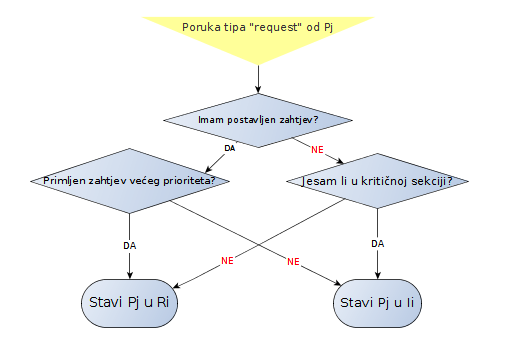
\includegraphics[width=10cm]{proces1}
			\end{figure}
			\item proces $P_i$ primi poruku tipa \textit{okay} od $P_j$:
			\begin{itemize}
				\item $R_i = R_i \setminus P_j$,
			\end{itemize}
		\end{itemize}
	\end{frame}
\begin{frame}
	%Problemi s kojima se algoritam susreo i uspješno riješio kako bi bio upotrebljiv.
	\begin{enumerate}
		\item Kako efikasno prepoznati koji procesi trenutno zahtjevaju ulaz u CS?
		\item Kako projektirati postavljenje zahtjeva za CS za procese iz grupe 2 (manje aktivne procese)?
		\item Kako omogućiti prijelaz iz grupe 2 u grupu 1 i obratno?
		\item Ukoliko proces ne zahtjeva odobrenje za ulazak u CS od svih procesa, kako osigurati svojstvo \textit{sigurnosti}? 
		\item Kako osigurati da prikupljanje informacija o trenutnom stanju sustava ne utječe na efikasnost poništavajući dobiveno poboljšanje?
	\end{enumerate}
\end{frame}

\begin{frame}
	\frametitle{Algoritam Lodha \& Kshemkalyany}
	\begin{itemize}
		\item Algoritam Lodha i Kshemkalyani je optimizirana verzija algoritma Ricarta i Agrawale za međusobno isključivanje.
		 \begin{itemize}
			\item sigurnost \checkmark
			\item pravednost \checkmark
			\item odsustvo izgladnjivanja \checkmark
		\end{itemize}
		\item Proces ne treba odobrenje svih procesa da uđe u kritični odsječak, već samo od onih čiji zahtjevi prethode njegovom zahtjevu prema prioritetu. 
	\end{itemize}
\end{frame}
\begin{frame}
	\frametitle{}
	\begin{itemize}
		\item Vrste poruka:
		\begin{itemize}
			\item REQUEST
			\item OKAY
			\item FLUSH
		\end{itemize}
		Poruke imaju vremenski žig.
		\item konkurentnost
		\item LQRi sadrži konkurentne zahtjeve posljednjeg zahtjeva Ri
	\end{itemize}
	
\end{frame}
\begin{frame}
	\frametitle{}
	\begin{itemize}
		\item Poruka \textbf{OKAY}:
		\begin{itemize}
			\item  dopuštenje od procesa koji nije zainteresiran za KO
			\item kolektivno dopustenje od procesa koji imaju zahtjeve viseg prioriteta
		\end{itemize}
		\item Poruka \textbf{FLUSH}
		\begin{itemize}
			\item odgovor procesa sa višim zahtjevima
			\item poruka procesu sa sljedećim najvecim prioritetom (ostalima OKAY)
		\end{itemize}
		\item Poruka \textbf{REQUEST}
		\begin{itemize}
			\item nema konkurentnih zahtjeva 
			\item ima konkurentnih zahtjeva, request nižeg služi kao okay
		\end{itemize}
	\end{itemize}
	Da bi ušao u KO, proces pošalje $(N-1)$ poruka request, a primi $(N - |$broj konkurentnih zahtjeva$|$) odgovora u obliku \textit{okay/flush}
	
\end{frame}
\begin{frame}
	\frametitle{Algoritam Maekawa}
	\begin{itemize}
		\item prvi algoritam za međusobno isključivanje zasnovan na kvorumu
		\begin{itemize}
			\item proces ne zahtijeva dopuštenje od svih ostalih procesa nego samo od nekog podskupa procesa
			\item podskupovi zadovoljavaju pravilo $\forall$ i, j:1$\leq$i,j$\leq$N $\Rightarrow$ Ri$\cap$ Rj$\neq$ $\emptyset$ i svaki skup se naziva \textit{kvorum}
		\end{itemize}
		\item Skup kvoruma u algoritumu Maekawa konstruiran je tako da zadovoljava sljedeće uvjete: 
		\begin{itemize}
			\item [M1] ($\forall$ i,j : i $\neq$ j $\Rightarrow$ Ri $\cap$ Rj $\neq$ $\emptyset$)
			\item [M2] ($\forall$ i : 1$\leq$i$\leq$N $\Rightarrow$ Si $\in$ Ri)
			\item [M3] ($\forall$ i : 1$\leq$i$\leq$N $\Rightarrow$ $\mid$ Rt $\mid$ = K)
			\item [M4] Svaki proces nalazi se u K kvoruma
		\end{itemize}
		
		\item Maekawa je koristio teoriju projektivnih ravnina za konstrukciju kvoruma. Pokazao je da vrijedi N = K(K - 1) + 1. Iz te relacije slijedi $\mid$ Ri $\mid$ =  $\surd$N.
		
	\end{itemize}
\end{frame}

\begin{frame}
	\frametitle{Primjeri skupa kvoruma}
	
	\begin{table}[H]
		\centering
		\caption{Primjer skupa kvoruma koji zadovoljavaju uvjete algoritma Maekawia gdje je K=2}
		\label{my-label}
		\begin{tabular}{|l|l|}
			\hline
			& $R_1$ = $\left\{\text{1, 2}\right\}$  \\
			K=2, N=3    & $R_2$ = $\left\{\text{2, 3}\right\}$ \\ 
			& $R_3$ = $\left\{\text{1, 3}\right\}$ \\ \hline
		\end{tabular}
	\end{table}
	
	\begin{table}[H]
		\centering
		\caption{Primjer skupa kvoruma koji zadovoljavaju uvjete algoritma Maekawia gdje je K=3}
		\label{my-label}
		\begin{tabular}{|l|l|}
			\hline
			& $R_1$ = $\left\{\text{1,2,3}\right\}$  \\
			& $R_2$ = $\left\{\text{2,4,6}\right\}$  \\
			& $R_3$ = $\left\{\text{3,5,6}\right\}$  \\
			K=3, N=7    & $R_4$ = $\left\{\text{1,4,5}\right\}$ \\ 
			& $R_5$ = $\left\{\text{2.5.7}\right\}$  \\
			& $R_6$ = $\left\{\text{1,6,7}\right\}$ \\
			& $R_7$ = $\left\{\text{3,4,7}\right\}$  \\\hline
		\end{tabular}
	\end{table}
	
	
\end{frame}

\begin{frame}
	\frametitle{Pseudokod}
	\begin{enumerate}
		\item \textbf{Zahtijevanje kritičnog odsječka}
		\begin{itemize}
			\item Proces Si šalje REQUEST(i) svim procesima koji se nalaze u istom kvorumu Ri
			\item  Kada proces Sj primi REQUEST(i), šalje REPLY(j) procesu Si, samo ukoliko poruka REPLY nije već poslana nekom procesu inače stavlja u red čekanja REQUEST(i) za kasniju obradu.
		\end{itemize}
		
		\item \textbf{Izvršavanje kritičnog odsječka}
		\begin{itemize}
			\item  Proces Si ulazi u kritični odsječak kada primi poruku REPLY od svakog procesa u kvorumu Ri.
		\end{itemize}
		
		
		\item \textbf{Izlazak iz kritičnog odsječka}
		\begin{itemize}
			\item Proces Si šalje poruku RELEASE(i) svakom procesu u kvorumu Ri
			\item Kada proces Sj primi RELEASE(i) od Si, šalje REPLY sljedećem procesu koji je u njegovom redu čekanja te ga miče iz reda. 
			Ukoliko je red prazan proces ažurira svoje stanje tako da tako da može poslati poruku REPLY kao odgovor na REQUEST poruku
		\end{itemize}
	\end{enumerate}
\end{frame}

\begin{frame}
	\frametitle{Svojstva}
	\begin{itemize}
		\item Na prethodno opisan način postiže se međusobno isključivanje
		\item Ali može doći do zastoja (deadlock) zato što proces može biti blokiran od strane drugih procesa
		\item Poruke REQUEST nisu prioritizirane s obzirom na vrijeme slanja. Dakle, proces može poslati zahtjev procesu i kasnije prisiliti zahtjev većeg prioriteta da čeka (nije zadovoljeno svojstvo pravednosti). 
	\end{itemize}
\end{frame}


\begin{frame}
	\frametitle{Dodatne poruke}
	\begin{itemize}
		\item FAILED, INQUIRE, YIELD
	\end{itemize}
	
	
	\begin{enumerate}
		\item Kada proces Sj blokira zahtjev REQUEST(ts, i) \footnote{\texttt{ts je vremenski žig (timestamp)}} procesa Si zato što je već dao dopuštenje procesu Sk, proces Sj šalje procesu Si poruku FAILED(j) ukoliko Si ima manji prioritet od procesa Sk. Inače proces Sj šalje procesu Sk poruku INQUIRE(j).
		\item Kao odgovor na primljenu poruku INQUIRE(j) od procesa Sj, proces Sk šalje poruku YIELD(k) procesu Sj nakon što je primio poruku FAILD od nekog procesa u svom kvorumu i ukoliko je poslao YIELD poruke, a nije primio REPLY kao odgovor.
		\item Kada proces Sj primi YIELD(k) poruku od procesa Sk, proces Sj sprema zahtjev porocesa Sk na pravo mjesto u svom redu procesa koji čekaju i šalje REPLY(j) poruku procesu koji je prvi u redu.
	\end{enumerate}
\end{frame}

\end{document}